\documentclass[10pt]{article}

\usepackage[a4paper, left=2cm, right=2cm]{geometry} % A4 paper size and thin margins

\usepackage{xcolor} % Required for specifying custom colours
\definecolor{grey}{rgb}{0.9,0.9,0.9} % Colour of the box surrounding the title

\usepackage{graphicx}
\usepackage[colorlinks=true, allcolors=black]{hyperref}
\usepackage{amsmath}
\usepackage{indentfirst}
\setlength{\parindent}{2em}


\usepackage[utf8]{inputenc} % Required for inputting international characters
\usepackage[T1]{fontenc} % Output font encoding for international characters
\usepackage[sfdefault]{ClearSans} % Use the Clear Sans font (sans serif)
%\usepackage{XCharter} % Use the XCharter font (serif)

\begin{document}
%----------------------------------------------------------------------------------------
%	TITLE PAGE
%----------------------------------------------------------------------------------------

\begin{titlepage} % Suppresses displaying the page number on the title page and the subsequent page counts as page 1
	
	%------------------------------------------------
	%	Grey title box
	%------------------------------------------------
	
	\colorbox{grey}{
		\parbox[t]{1.1\textwidth}{ % Outer full width box
			\parbox[t]{1.02\textwidth}{ % Inner box for inner right text margin
				\raggedleft % Right align the text
				\fontsize{34pt}{40pt}\selectfont % Title font size, the first argument is the font size and the second is the line spacing, adjust depending on title length
				\vspace{0.7cm} % Space between the start of the title and the top of the grey box
				
				< Journey Assistant >\\
              Feasibility Analysis Report\\
                Version 1.0\\
				
				\vspace{0.7cm} % Space between the end of the title and the bottom of the grey box
			}
		}
	}
	
	\vfill % Space between the title box and author information
	
	%------------------------------------------------
	%	Author name and information
	%------------------------------------------------
	
	\parbox[t]{1\textwidth}{ % Box to inset this section slightly
		\raggedleft % Right align the text
		\large % Increase the font size
		{\Large Group Member}\\[4pt] % Extra space after name
        Yiwen Song\\
        Zhihui Xie\\
        Weizhe Wang\\
        Huangfei Jiang\\
        Haoping Chen\\
		% Institution Name\\[4pt] % Extra space before URL
		% \texttt{LaTeXTemplates.com}\\
		
		\hfill\rule{0.2\linewidth}{1pt}% Horizontal line, first argument width, second thickness
    }
    
	
\end{titlepage}

\newpage

\begin{center}
    {\LARGE Modification History}
    
    \begin{tabular}{|c|c|c|c|} 
        \hline 
        Date&Version&Description&Author\\
        \hline  
        2019-04-06&1.0&The first version of this document.&Zhihui Xie \& Haoping Chen\\
		\hline 
		 & & & \\
		\hline
		& & & \\
		\hline
		& & & \\
		\hline
    \end{tabular}    
\end{center}

\newpage

\tableofcontents
\newpage


\section{Introduction}
\subsection{Purpose}
This document aims for giving an explicit exposition of why this program will work and what problems might occurs in our development. 

By doing complete and detailed market research, we posit situations where problems may occur and then propose our solutions in this report. This provides great convenience to our further development. It could be a very important reference for our developers. 

Besides, we expect readers such as the business managers of some travel portals and other potential cooperators can be convinced by this report. We will show the potential economic benefit as well as the risk behind the project.

This report will be reviewed and then works as a representation of responsibility for the head of the team.
\subsection{Background}
\paragraph{\underline{The Name of the Software System}}
The software system's temporary name is 'Journey Assistant', or 'JA' for short. 

\paragraph{\underline{The Proposer of the Task}} Zhihui Xie.

\paragraph{\underline{The Developers}} Yiwen Song (leader), Zhihui Xie, Weizhe Wang, Huangfei Jiang, and Haoping Cheng.

\paragraph{\underline{The Aimed Users}} People who find it hare to make travel plans or simply have no enough time to travel.

\paragraph{\underline{The Relationship With Other Systems or Associations}} There will be other systems involved in our system as third-party service, while the system will be relatively independent at first by using open-source APIs. When the system grows huge, we will seek cooperations with other systems or associations.

\subsection{Definition}
Here we list some terms or abbreviations we will use in this file.

\begin{center}
\begin{tabular}{|c|c|c|} 
	\hline 
	Abbreviation&Term&Implication\\
	\hline  
	JA&Journey Assistant&The Name of our Project\\
	\hline 
	 &Android&An OS Developed by Google\\
	\hline
\end{tabular}    
\end{center} 

\subsection{Bibliography}
\begin{itemize}
  \item[(1)] <Feasibility Study Report> (GB8567-88)
  \item[(2)] <Object Oriented Software Engineering (Version 3)> (Tsinghua University Press)
  \item[(3)] <Object Oriented Software Engineering Practice Guidelines>
\end{itemize}

\section{Presupposition}
This part will provide some presuppositions for the project to do feasibility study.

\subsection{Requirement}
\subsubsection{Functional Requirement}
Our system includes but not limited to these functions: 

\begin{itemize}
  \item Register and Log in of Users.
  \item Railormade Itinerary Recommendation.
  \item Travel Experience Simulation.
  \item Itinerary Sharing.
  \item Schedule Creating.
\end{itemize}

Users who are logged in can manage their personal information, which can be of reference significance for further functions. Our journey assistant provides itinerary recommendation and travel simulation in a highly personalized manner, making users feel like they are actually placed in a real situation. And a really interesting thing is, with the journey assistant, users can experience the journey on his or her phone, making decisions and getting feedback on the experience. Users can consider the application as a travel reference or a story book where you can truly place yourself into a journey. 

Besides, we also devote ourselves to build this software a platform where users can truly share their itineraries and considerations in regard to how they plan their journey. Users can share their itineraries when their simulated travelling is over, or star others' travel schedule. There will be a lot of fun.

\subsubsection{Performance Requirement}
\paragraph{\underline{Treatment Capacity of the System}} The maximum concurrent users our system may support is around 1000. To meet the demand of itinerary recommendation algorithm, we need a powerful server that allows over 1000 concurrent events. There could be massive computing task, hence the system should be surely computing-capable.

\subsubsection{Input}
\paragraph{\underline{User Information}}
\begin{itemize}
  \item[1.] Source: User register.
  \item[2.] Type: Complex data type.
  \item[3.] Number: Over 50000.
  \item[4.] Component: User ID (integer), user name (string), phone number (string), email (string), and other preference information.
\end{itemize}

\paragraph{\underline{Travel Expectation}}
\begin{itemize}
  \item[1.] Source: User.
  \item[2.] Type: Complex data type.
  \item[3.] Number: Over 50000.
  \item[4.] Component: Travel time (string), number of travelers (integer), travel style (string), destination expectation (string) and cost expectation.
  \item[5.] Frequency: High. 
\end{itemize}

\paragraph{\underline{Message Logging}}
\begin{itemize}
  \item[1.] Source: User.
  \item[2.] Type: Complex data type.
  \item[3.] Number: Over 200000.
  \item[4.] Component: Message ID (integer), Message content (string), time (time), and user ID (integer).
  \item[5.] Frequency: High.   
\end{itemize}

\subsubsection{Output}
\paragraph{\underline{Recommended Itinerary}}
\begin{itemize}
  \item[1.] Implication: The itinerary automatically generated by the recommendation system.
  \item[2.] Frequency: High.
  \item[3.] API: Amap.  
  \item[4.] Object: Users who need itinerary recommendations. 
\end{itemize}

\paragraph{\underline{Travel Experience Feedback}}
\begin{itemize}
  \item[1.] Implication: When the simulated travel starts, users will be presented real-time feedback on how the experience is depending on the choices users make.
  \item[2.] Frequency: High.
  \item[3.] API: No.  
  \item[4.] Object: Users who are experiencing a simulated travel. 
\end{itemize}

\paragraph{\underline{Message}}
\begin{itemize}
  \item[1.] Implication: Some system messages will be sent to users to notice them what to do next. Besides, users can receive messages of other users in our social community.
  \item[2.] Frequency: Depending on the scale of our social community. 
  \item[3.] API: No. 
  \item[4.] Object: Users. 
\end{itemize}

\subsubsection{Data Flow and Processing Flow}
\begin{center}
  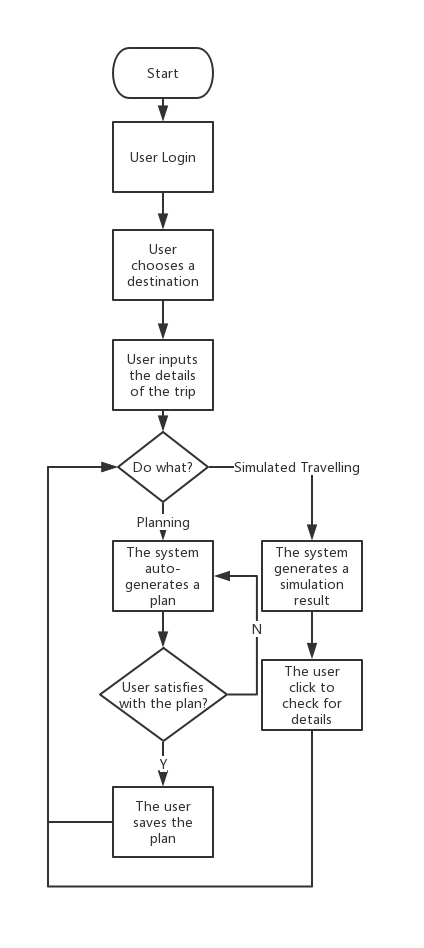
\includegraphics[width=6cm]{test.png}
\end{center}

\subsubsection{Security and Confidentiality}
\begin{itemize}
  \item[1.] Users can only access to their own information in the user form.
  \item[2.] The encryption method of user keyword needs further discussion.
  \item[3.] The information exchange when interacting with other external systems will be protected, while the specific method still needs discussion later.
\end{itemize}

\subsubsection{Deadline}
2019.6.23

\subsection{Purpose}
People loves travelling, while it would not be that easy to simply pack our bags and check out of our normal life. We need a perfect reason to persuade our empty wallet, tight schedule, and poor execution. Even if we are well-qualified, our lazy brain will tell us that itinerary is something it can not bear. Natually, we will in the end choose to stay at home during holidays. Is there any alternative solution?

The purpose of our project is simple but huge: to make trip planning easier and more interesting. An experience-oriented journey assistant is therefore designed. For those who find it hard to make travel plans or simply have no enough time, the application may help. It provides itinerary recommendation and travel simulation in a highly personalized manner, making users feel like they are actually placed in a real situation. And a really interesting thing is, with the journey assistant, users can experience the journey on his or her phone, making decisions and getting feedback on the experience. Users can consider the application as a travel reference or a story book where you can truly place yourself into a journey.

\subsection{Condition, Supposition and Limitation}
\paragraph{\underline{The Minimum Recommended Operating Life of the System}} 
Around 3 years.

\paragraph{\underline{Time for Comparison of System Options}}
At least 3 months. (There will be a lot of algorithm-related work to test)

\paragraph{\underline{Sources and Restrictions on Investment or Funds}}
It will depends on the potential investors and our group.

\paragraph{\underline{Restrictions on Law and Policy}}
Since there may be a lot of interconnection service, we need to take more care about law and policy. We will observe commercial ethics, avoiding to use other systems' information without permission.

\paragraph{\underline{Conditions on Developing/Run-time Environment or Hardware/Software}}
Apart from some conventional servers to deal with data and security, we need one high-performance server to meet the demand of our recommendation computing task. We also need some Android phones for testing since our development environment is on Android.

\paragraph{\underline{Available Information and Resources}}
There are massive network resources on Android development, server deployment, and etc.

\paragraph{\underline{Deadline for the System to Come Into Operation}}
Summer, 2019.

\subsection{Method of Feasibility Study}
The feasibility study goes on along with our group discussion. We will relate our own travelling experience to modify the system. 

Besides, we will do some survey on campus and Internet. By trying to find the true pain points of our target users, we dig deep into the defect of existing products and then do perfection.

Another tactic is to release a beta in a small scale. We receive feedbacke and then improve our system.

\subsection{Evaluation Criteria}
The main criteria are as follows:

\begin{itemize}
  \item[1.] Cost of the system development.
  \item[2.] Development time.
  \item[3.] Difficulty of operation and maintenance.
  \item[4.] User satisfaction. 
\end{itemize}

\section{Existing System Analysis}
Current tourism platform like Xiecheng has similar system on recommending travel. The recommendation is based on the inputted information, such as target city, number of travelers, number of days to travel, travel budget, and so on. However, most of current recommending systems collect the travelers’ demand and let several travel advisers to help you arrange your trip. They may contact the travelers by phone or by email and charge them after traveler have agreed on the trip they design. It may be bothering to receive ceaseless phones and emails about the itinerary. Also, when the travelers have paid their consulting fee, the travel adviser may not responsible for any change on the itinerary. 

\subsection{Data Flow and Processing Flow}
Take travel recommendation on Xiecheng website as example. Data flow and processing flow are as follows:

\begin{center}
  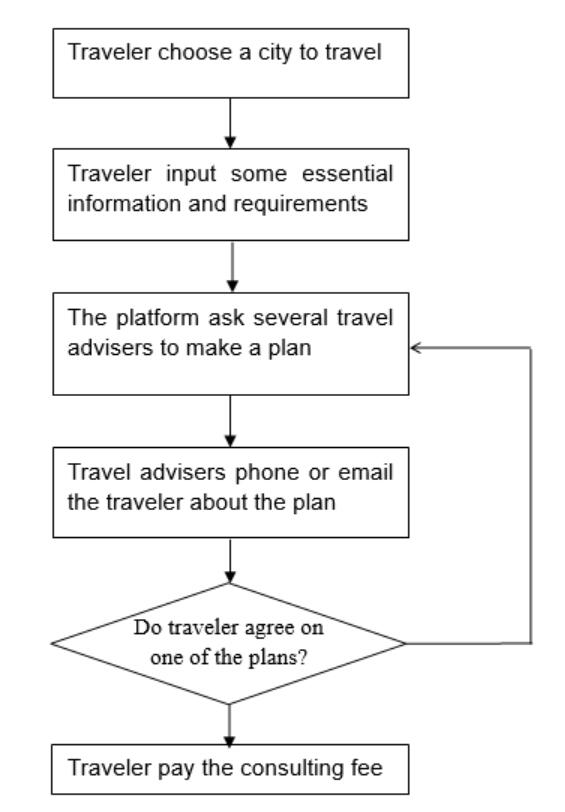
\includegraphics[width=6cm]{1.jpg}
\end{center}

\subsection{Working Load} 
Since the system helps travelers plan their tour for a given destination, it involves consulting travel advisers, travel advisers then plan the travel plan and inform the travelers by phone or email, which will all be done manually. The working load is comparatively large.

\subsection{Expenditure}
Large amount money spent on paying the salary of travel advisers. Travelers also spend a long time waiting for the adviser to give a reasonable plan.

\subsection{Personnel}
\begin{itemize}
  \item[1.] A big number of travel advisers with professional skills on tourism planning.
  \item[2.] Several experts on maintaining the website.
  \item[3.] Several employees to deal with complaints from travelers. 
\end{itemize}

\subsection{Devices}
\begin{itemize}
  \item[1.] A website
  \item[2.] Cellphone or email to communicate 
\end{itemize}

\subsection{Limitation}
Firstly, all the recommendation is done by manual work, so a large amount of advisers is needed, which increase the cost of the system. Secondly, travelers can not get timely recommendations for they have to wait for travel advisers to make plans and communicate with them. Thirdly, the traveler is expected to receive several phones, which is quite bothering. 

Since all recommendations are made manually, time for planning a trip for a single adviser will not decrease dramatically due to a higher level mastery of their skills. After all, travel demands vary among tourists. So the number of advisers and time that one traveler is expected to wait will not decrease markedly. Also, the procedure of travel adviser communicating with travelers can not be omitted. They may negotiating about some details of the travel plan. So it’s quite impossible to break the limits with some improvement of the current system.

\section{Proposed System}
\subsection{Some Explainations}
The system provides itinerary recommendation and travel simulation in a highly personalized manner, making users feel like they are actually placed in a real situation. And a really interesting thing is, with the journey assistant, users can experience the journey on his or her phone, making decisions and getting feedback on the experience. Users can consider the application as a travel reference or a story book where you can truly place yourself into a journey.

To meed the requirements mentioned in Chapter 2, we need to achieve these aspects:

\paragraph{\underline{Well-designed Algorithm}}
Since one of our most prominent is itinerary recommendation, we need a well-designed algorithm to provide highly customized itinerary for any conditions. It also needs to be fast to work real-time. Thankfully, some of our group members have related knowledge on combinatorial optimization and graph theory.

\paragraph{\underline{High-performance Server}}
As mentioned before, we may deal with a lot of computing. Hence, the deployment of high-performance servers is quite important. However, it is always a tricky problem that how these servers are deployed to maximize the operating efficiency. We will work on it and seek some perfessional advice.

\paragraph{\underline{Good Teamwork}}
Although we are a small team in the beginning, good teamwork still matters for our project. It will certainly boost the development and help us meet the deadline.

\subsection{Data Flow and Processing Flow}

\begin{center}
  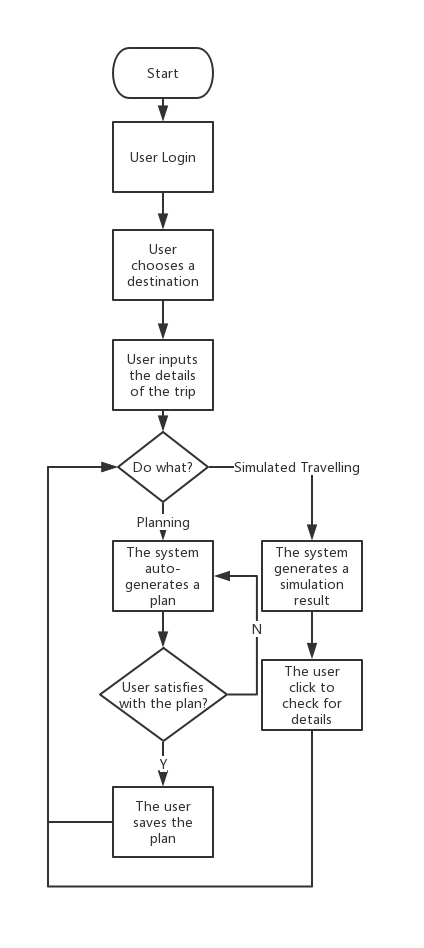
\includegraphics[width=6cm]{test.png}
\end{center}

\subsection{Improvement}
Previously carried out surveys shows that we have two different choices now to make a detailed travel plan.

The first one is to get armed with various travel applications, such as Mafengwo, Xiechen, Dazhongdianping, and etc. Although all of them have their own travel service, we usually have to 
refer to different applications to make the plan exhaustive. In other word, it lacks connection such as one between accommodation and catering, which makes the whole planning experience terrible. 

Though there is an alternative. Some trip planning applications appear in recent years, such as Google Trips and Xingchengzhushou. These applications are trying to provide door to door service on trip planning, with all essential factors considered. The integration of functions truly bring great progress, but something important is still missing. These newly-born applications provide too much information to balance the software logic well. Take Google Trips for example, when I want to choose a reservation to visit, I will sometimes be overwhelmed by the massive recommendations and forget where my hotel is and whether I could make it getting back to my hotel before dark. Different functions are separated, so I could not focus on simply planning what to do next. 

Hence, to reach our purpose, we make improvement in two aspects. First, our system provides more travel information, and integrates them as a whole. Our users would no longer need to use other applications when making the plan, and it is natural for them to make choices on things like accommodation. Another improvement is about customization. Existing systems have no similar service that provides intuitive experience on what would happen when the user chooses a itinerary. Since the user receives only data instead of true feelings, travel planning can be really boring and unrealistic. So we want to let users decide everything, and our system only provides them a simulation environment. This would definitely make things easier and more interesting.

\subsection{Impact}
\subsubsection{Impacts on Devices}
To support the proposed system, we need more than normal servers. Several powerful GPUs should be deployed to achieve itinerary recommendation function, which requires deep learning algorithm to handle. To be specific, we need at least 4 NVIDIA GEFORCE RTX 2080 Ti for calculation.

\subsubsection{Impacts on Software}
Apart from special hardware support, we also need software support to deal with our recommendation service. 

By comprehensive consideration, we choose 'Submarine' -- a new subproject of Apache Hadoop which allows infra engineer / data scientist to run deep learning applications (Tensorflow, Pytorch, etc.) on resource management platform (like YARN). The project can be directly deployed in our existing system based on Hadoop backend.

\subsubsection{Impacts on Users}
Because our application takes aim at ordinary users, we do not want to increase the learning cost. So the only impact on users is to ask them think different.

\subsubsection{Impacts on Run-time Process}

\subsubsection{Impacts on Development}
\begin{itemize}
  \item[a.] To support our proposed system, users should send feedback on user experience during the beta phase.
  \item[b.] Except user information, the database for the system need to store information of destination, accommodation, catering, and etc. These data will come from public resource or other company.
  \item[c.] To develop and test our system, we need a basic Linux platform with essential computing capacity. Service deployment is quite tricky here, so we may need another small server for our development.
  \item[d.] In regard to security and safety, we think that the best way is to develop as individually as possible. Besides, for some outsourcing work, we will cautiously draw up a contract, esperically on the default part. 
\end{itemize}

\subsubsection{Impacts on Location and Facility}
A small room, or even part of it, is enough for our project.

\subsubsection{Impacts on Expenditure}
The expenditure mainly includes these three parts: development, design, and maintenance.

\paragraph{\underline{Development}}
Since the main developers are ourselves, we can lower the expenditure as much as possible, depending on how focus we are. But afterall, we still need some outsourcing development, which may cost thousands or more.

\paragraph{\underline{Design}}
Art design is really beyond our ability, so we seek help from others. It could be another thousand to pay the art design.

\paragraph{\underline{Maintenance}}
By comprehensive consideration, we will deploy our servers in the cloud. Take LeanCloud for example, it provides offer including basic cost 10 yuan / day and extra charges depending on the call volumes.

\subsection{Limitation}
The main limitation lies on the diversity. The system may not be able to provide massive content for users to choose. To ensure quality, we will only start from some popular destinations such as Beijing, and then do extend our business.

\subsection{Feasibility on Technical Condition}
\begin{itemize}
  \item[1.] The related algorithm is not hard to realize, as machine learning grows really fast there years. The main functions of our system rely most on the inner factors, so it will not be a big issue as soon as we realize our algorithm.
  \item[2.] As mentioned before, we have 5 developers who are both able to work independently and collaborate well. Besides, professors in SJTU provide great help for us.
  \item[3.] We have a lot of time on weekends. Time should be good for us. 
\end{itemize}

\section{Alternative Solution}
Not available now. (We have no other systems that can compare with the proposed system.)

\section{Cost/Benefit Analysis}
\subsection{Cost}
Total cost: 5000 yuan (two-year period)
\subsubsection{Cost for Infrastructure (500 yuan / year)}
\paragraph{\underline{Hardware Devices}}
One server (The server is rent and we do not buy a server, 		also we can use our team members’ smart phones for software debugging and our computers for system construction.) 

\paragraph{\underline{Software}} Debug test software

\paragraph{\underline{Location}} Necessary place to locate hardware device

\paragraph{\underline{Maintenance}} Cost of fixing hardware and software

\subsubsection{Other Cost for One-off Investment (2000 yuan)}
\begin{itemize}
  \item[1.] Requirement research \& Design research
  \item[2.] Develop plan research \& Measure criterion research
  \item[3.]	Database construction
  \item[4.]	Cost for start project
  \item[5.]	Cost for technology management
  
\end{itemize}

\subsubsection{Non-One-off Investment (1000 yuan/year)}
\begin{itemize}
  \item[1.] Device rent and cost to maintain
  \item[2.]	Software rent and cost to maintain
  \item[3.]	Cost of data storage
  \item[4.]	Salary and premium for employers
  \item[5.]	Cost of the communication between team members
  \item[6.]	Other necessary usual expense such as the electric and water expense 
  
\end{itemize}

\subsection{Benefits}
Total benefit: 20000 yuan (two-year period)
\subsubsection{One-off Benefit}
Since we manage the system ourselves, there is no one-off benefit. 

\subsubsection{Non-one-off Benefit}
We can charge 1\% of the total travel cost of a traveler to use our system. Consider 1000 people use our system each year, and the average travel cost of a single traveler is 1000 yuan. The benefit is 10000 yuan one year.

\subsubsection{Immeasurable Benefit}
\begin{itemize}
  \item[1.]	The system can let traveler have a more timely and reliable recommendation of their travel.
  \item[2.]	The system is more flexible to users because they may also remake their plans during their travel. Thus users’ satisfication level rises.
  \item[3.]	Our immersive desciption of every spots attracts travelers, which stimulates traveling.
  
\end{itemize}

\subsection{Cost/Ratio Benefit}
According to similar software and our experience in development, we suppose the life cycle of this software is over 2 years. The total cost, including develop cost and maintain cost, is about ¥5,000.  The benefit from this product will come to 2000 yuan.

Therefore, we can calculate the ROI (ARR).

\begin{align*}
  ROI (Return on investment)/ARR (Accounting rate of return)&=(Anniversary benefit / Total cost) \times 100\%\\
  &=(7500 / 5000) \times 100\%\\
  &=125\%
\end{align*}

\subsection{Investment Return Period}

$$T=2000 / (20000 - 1500) = 1.3 (months)$$

\subsection{Sensibility Analysis}
\paragraph{\underline{Life Circle}} 2 years

\paragraph{\underline{Working Load}} Moderate

\paragraph{\underline{Working Type}} Proceesing with input data

\paragraph{\underline{Influence of Other Factors}} \subparagraph{Stability of the Server}
If the server stops working, our project will delay greatly, and the cost will rise roughly.  So the server must be opened all the time. Since we rent server for our project, if our server fails to start, we can connect the server provider and ask for compensation. The overall cost for this problem is not large.

\subparagraph{Persistence of Data}
If the date can’t be operate correctly, the whole project may face risk and the system may lose most of its functions. In order to save the relative data of the project more safely, we use the some outer storage to store the data. While the data is destroyed because of some accident, we can manually recover the date.

\subparagraph{Security of Data}
If our competitors thief our important data, our whole will face difficult. Our products couldn’t be sold out, and we may suffer deficit. 

\subparagraph{Similar Products from the Counterpart}
If our competitors release a similar product, our profit may be influence. We shall release our product before our competitors. 

\subparagraph{Resource}
Make full use of the resource and cut some unnecessary waste can I increase the profit.

\subparagraph{Team members}
Our plan shall be modified and the project must be delayed. So we must have a more flexible project schedule. The health of team members is critic to our project. 

\subparagraph{Market Demand}
If the market requirement is not large as we supposed, our profit will drop dramatically. So we have to provide something different to the users, like immersive experience on each scenic spot, smooth usage experience and a beautiful UI.

\section{Other Social Factors}
\subsection{Law-based Factors}
The system is fully in charge of our group, so there’s no problem of contractual liability.

The technology of our project is developed by ourselves or from open-sourced community, so there’s no infringement of copyright.

Whether using this system or not is depend on user, there’s no problem of debt and proprietorship.

\subsection{Usability-based Factors}
The system is mainly focused on urban residents, and at initial stage, we will recommend our system to our friends, classmates and their family. People who use our system are mainly well-educated and it’s not difficult for them to figure out how to use our system.

Our system is interactive friendly and easy to use, there’s also a user guide. The immersive travel experience is attractive. Besides, our system use APP as client side, which can attract users, too.

\section{Conclusion}
We can get a conclusion from the all the analyze aboved: we can start the project at once.
\end{document} 